\documentclass[11pt]{article}
\usepackage[margin=1in]{geometry}
\usepackage{graphicx}
\usepackage{booktabs}
\usepackage{multirow}
\usepackage{amsmath}
\usepackage{tikz}
\usetikzlibrary{arrows.meta, positioning}
\usepackage{float}
\usepackage{hyperref}
\usepackage{enumitem}

\newcommand{\celsius}{\ensuremath{^\circ\mathrm{C}}}

\title{AgriFrost-AI Progress Report\\F3 Innovate Frost Risk Forecasting Challenge}
\author{AgriFrost-AI Team}
\date{\today}

\begin{document}
\maketitle
\begin{abstract}
This report documents the AgriFrost-AI system submitted to the F3 Innovate Frost Risk Forecasting Challenge. We construct a fully reproducible, short-term frost risk forecasting pipeline that ingests 15~years of hourly CIMIS data, engineers both temporal and spatial features, and trains a diverse set of machine learning and graph-based models across four forecast horizons (3, 6, 12, 24\,h). The study emphasizes calibrated probabilistic outputs, strict temporal integrity, spatial generalization via Leave-One-Station-Out (LOSO) evaluation, and actionable decision guidance for growers. We benchmark the 2\(\times\)2+1 ABCD matrix of feature regimes, quantify performance degradation across horizons and matrices, and analyze the role of near-surface variables—particularly soil temperature gradients and moisture diagnostics—in driving early warning skill. The manuscript concludes with an outlook on synoptic-scale integration using ERA5/HRRR predictors.
\end{abstract}

\tableofcontents
\clearpage

\section{Introduction}
Frost remains one of the most damaging weather risks for California specialty crops, especially during bloom, when a single radiative event can eliminate annual revenue. The F3 Innovate Frost Risk Forecasting Challenge provides a production-aligned evaluation setting: participants must produce calibrated frost probabilities and temperature forecasts at 3, 6, 12, and 24\,h horizons, quantify calibration, and prove spatial generalization with Leave-One-Station-Out (LOSO) evaluation. AgriFrost-AI focuses on three practical questions: (i) how to design features that respect near-surface physics while remaining usable for machine learning under extreme class imbalance, (ii) how to incorporate neighbor information to capture cold-air pooling without exploding runtime, and (iii) how to translate calibrated probabilities into standard operating procedures (SOPs) for growers rather than mere rankings.

The main contributions of this report are:
\begin{enumerate}[leftmargin=*]
    \item A unified frost-risk dataset covering 18 CIMIS stations (2010--2025) with comprehensive quality-control analysis.
    \item The ABCD feature matrix that crosses single vs.\ multi-station scope with raw vs.\ engineered features, together with a systematic comparison of tree ensembles and spatio-temporal neural networks.
    \item Strict LOSO evaluation demonstrating the spatial generalization gains of neighborhood aggregation across all horizons.
    \item A decision-support mapping that links calibrated frost probabilities and temperature forecasts to concrete intervention thresholds for growers.
\end{enumerate}

\section{Related Work}\label{sec:related}
Short-term frost forecasting has long been explored in agrometeorology, numerical weather prediction, and machine learning. Traditional methods rely on empirical formulas, statistical regressions, or downscaled mesoscale models (for example WRF) to represent radiative cooling, surface energy balance, and cold-air drainage. With the growing availability of automatic weather stations and reanalyses, data-driven approaches based on random forests, gradient-boosted trees, and deep networks combine satellite imagery, terrain descriptors, and reanalysis fields to build high-resolution frost-risk maps. Our work differs by (i) benchmarking a diverse model zoo on a single standardized dataset and metric suite, (ii) modeling neighbor aggregation explicitly rather than via gridded interpolation so that cold-air pooling and inversion layers are observable, and (iii) analyzing calibrated probabilities from the standpoint of decision support for growers.

\section{Data and Study Region}\label{sec:data}
\subsection{Observation Sources and Spatial Coverage}
We use hourly observations from the California Irrigation Management Information System (CIMIS) at 18 stations spanning the Central Valley and adjacent foothills from Sacramento down to Bakersfield. The network covers cold-air pooling basins, slope breaks, and high-evapotranspiration croplands, allowing us to test models under diverse microclimates. Figure~\ref{fig:stationmap} maps all stations. The record spans 2010--2025 and contains \(\sim 2.36\) million hourly entries. Each row includes air temperature, dew point, relative humidity, wind speed and direction, solar radiation, soil temperature, vapor pressure, and reference evapotranspiration (ETo), along with CIMIS quality-control (QC) flags. Station metadata—ID, location, elevation, ground cover, ETo flag, start/stop dates—is appended for spatial aggregation and LOSO grouping. All raw data and processing scripts reside in the public repository for traceability.

\begin{figure}[H]
    \centering
    \includegraphics[width=0.72\textwidth]{figures/station_distribution_map.png}
    \caption{Spatial distribution of the 18 CIMIS stations used in this study.}
    \label{fig:stationmap}
\end{figure}

\subsection{Frost Event Distribution and Seasonality}
Frost events are labeled when the observed temperature falls below \(0~\celsius\). Figure~\ref{fig:frost_month} shows the monthly climatology: December and January account for roughly 77\% of all events, February contributes about 13\%, and the remaining months are almost frost-free. Overall, frost represents only 0.87\% of the hourly records, making the task extremely imbalanced. This motivates the use of PR-AUC and calibrated probabilities when evaluating classifiers and setting decision thresholds.

\begin{figure}[H]
    \centering
    \includegraphics[width=0.85\textwidth]{figures/frost_events_by_month.png}
    \caption{Monthly distribution of frost events (2010--2025, all stations combined).}
    \label{fig:frost_month}
\end{figure}

\subsection{Core Observed Variables}
The CIMIS sensors provide the near-surface variables that drive frost physics:
\begin{itemize}[leftmargin=*]
    \item \textbf{Air temperature} is the target for both the binary frost label and the regression head.
    \item \textbf{Dew point and relative humidity} describe atmospheric moisture and saturation, which control condensation and radiative cooling efficiency.
    \item \textbf{Wind speed/direction} capture boundary-layer mixing and advection; weak winds indicate favorable conditions for radiative frosts.
    \item \textbf{Solar radiation} governs daytime heat storage and the energy available for nocturnal release.
    \item \textbf{Soil temperature} reflects the exchange of heat between the surface and the near-surface layer.
    \item \textbf{Vapor pressure and ETo} summarize the atmospheric demand for moisture and correlate with nighttime cooling rates.
\end{itemize}
These variables form the basis for lagged features, rolling statistics, harmonic encodings, and neighbor aggregations.

\subsection{Data Quality and QC Overview}
Every observation carries CIMIS QC flags. We keep only “blank/pass” and “Y” flags, treat all others (M/Q/R/S/P) as missing, and remove sentinel values such as \(-6999\). After QC, only 1.71\% of rows have at least one unusable key variable, indicating overall high data quality. Figure~\ref{fig:qc_station} shows the station-level share of bad records—issues are scattered rather than concentrated. At the variable level (Figure~\ref{fig:qc_variable}), ETo contributes 27.8\% of the bad records, soil temperature 20.4\%, and wind speed about 10.1\%. Air temperature accounts for just 6.2\% of bad QC entries (roughly 0.1\% of all rows), underscoring the suitability of this dataset for frost analysis.

\begin{figure}[H]
    \centering
    \includegraphics[width=0.70\textwidth]{figures/qc_bad_by_station.png}
    \caption{Share of low-quality (Bad QC) records by station.}
    \label{fig:qc_station}
\end{figure}

\begin{figure}[H]
    \centering
    \includegraphics[width=0.82\textwidth]{figures/qc_bad_by_variable.png}
    \caption{Distribution of low-quality records across meteorological variables.}
    \label{fig:qc_variable}
\end{figure}

\section{Methods}\label{sec:methods}
This section covers preprocessing, feature engineering, the ABCD matrix, model families, data splits, and evaluation metrics.

\subsection{Preprocessing Workflow}
A unified \texttt{DataCleaner} pipeline executes the following steps:
\begin{enumerate}[leftmargin=*]
    \item \textbf{Data ingestion and time normalization}: merge station CSV/Parquet files, convert timestamps to local solar time, and append station metadata.
    \item \textbf{QC and sentinel handling}: parse all \texttt{qc\_} fields, keep only pass/Y flags, drop the rest, and replace sentinel values such as \(-6999\) with missing.
    \item \textbf{Missing-value handling}: forward-fill short gaps per station, retain masks for long gaps or critical variables so that models are aware of observational incompleteness.
    \item \textbf{Label generation}: simultaneously create frost/no-frost labels and temperature targets for the 3/6/12/24\,h horizons, ensuring every experiment shares the same targets.
\end{enumerate}

\subsection{Feature Families and Matrix Cells}
Feature engineering follows a 2\(\times\)2+1 matrix that combines single vs.\ multi-station scope with raw vs.\ engineered representations (Table~\ref{tab:matrix}). Matrix~C typically performs best: neighbor soil-temperature gradients, dew-point spreads, and vapor-pressure deficits deliver the strongest early-warning signals across all horizons. Matrix~B is dominated by lag statistics, while Matrix~A (raw single-station signals) can miss nocturnal inversions. Matrix~D adds high-cardinality engineered features on top of spatial aggregation but shows diminishing marginal gains at the current noise levels.

\begin{table}[H]
    \centering
    \small
    \caption{ABCD matrix definition.}
    \label{tab:matrix}
    \begin{tabular}{llll}
        \toprule
        Cell & Spatial scope & Feature composition & Default models \\
        \midrule
        A & Single station & 12 raw CIMIS variables + harmonics & LightGBM, CatBoost \\
        B & Single station & Top 175 engineered features (lags, rolling stats, anomalies) & LightGBM, XGBoost, CatBoost \\
        C & Radius aggregation (20--200\,km) & Raw + 288 neighbor statistics + missingness cues & LightGBM, ST-GCN, DCRNN \\
        D & Radius aggregation + FE & Cell~B features + neighbor bundle (534+ features) & CatBoost, XGBoost, ensembles \\
        \bottomrule
    \end{tabular}
\end{table}

Matrix~C retains 534 predictors (12 local measurements, 288 neighbor statistics, temporal encodings, and missingness indicators). The most impactful near-surface signals stem from neighbor soil-temperature gradients, dew-point spreads, and vapor-pressure deficits. Matrix~B is dominated by engineered lag statistics, whereas Matrix~A relies primarily on raw air temperature and relative humidity, making it less robust during nocturnal inversions. Matrix~D adds the engineered stack to the spatial neighborhood but shows diminishing calibration gains without additional synoptic cues.

\subsection{Feature Selection and Importance Analysis}\label{subsec:feature_selection}
The full ABCD configuration yields about 298 candidate features (temporal encodings, lags, rolling windows, derived meteorology, station metadata, and neighbor aggregates). To control runtime and avoid noise, we apply a two-stage selection strategy:
\begin{enumerate}[leftmargin=*]
    \item \textbf{Full-feature baseline}: train LightGBM on Matrix~B for the 12\,h horizon with all features, then export \texttt{frost\_feature\_importance.csv} and \texttt{temp\_feature\_importance.csv} containing raw scores, relative percentages, and cumulative percentages.
    \item \textbf{Cumulative cutoff}: order features by importance and select the smallest \(k^\star\) with cumulative importance \(\ge 90\%\). Empirically \(k^\star\approx175\) (about 60\% of the candidates). All subsequent experiments across matrices, horizons, and tasks use this shared 175-D feature space.
\end{enumerate}
The ROC-AUC and Brier deltas between full and reduced sets remain within \(10^{-3}\) for every horizon, while training/inference time drops by roughly 35--40\%. The per-horizon importance plots also highlight a long-tail distribution and make it easy to compare feature usage across classification and regression heads.

\subsection{Targets, Splits, and Leakage Prevention}
For every horizon \(h \in \{3,6,12,24\}\) we label frost if \(T_{t+h}<0~\celsius\) and regress on the expected temperature. Temporal splits follow a 70/15/15 chronology (train/validation/test) with the latest 15\% of each station reserved for hold-out evaluation. LOSO cross-validation removes an entire station from the training set, fits all preprocessing artifacts (scalers, PCA, neighbor caches) on the remaining stations, and evaluates on the held-out station to guarantee microclimate isolation. Within each split we preserve chronological order so that no target can see future information.

\subsection{Model Portfolio and Experiment Setup}
\begin{itemize}[leftmargin=*]
    \item \textbf{Tree ensembles}: LightGBM (primary), XGBoost, and CatBoost serve as the main probabilistic learners. Hyperparameters follow a common template (learning rate 0.05, 200--1000 estimators, depth 6--8, balanced class weights).
    \item \textbf{Graph/sequence baselines}: ST-GCN, DCRNN, and GRU/LSTM variants assess whether explicit spatial-temporal modeling yields incremental skill beyond engineered features.
    \item \textbf{Experiment orchestration}: A unified CLI orchestrates data processing, training, and evaluation for each matrix cell. Radius sweeps (20--200\,km) and horizon sweeps are scheduled with fixed random seeds to ensure comparability.
    \item \textbf{Metric logging}: Every run emits a standardized metric bundle, subsequently consolidated into the experiment catalogue used for the comparative analyses in Sections~\ref{sec:experiments} and \ref{sec:matrixcomparison}.
\end{itemize}

\subsection{Evaluation Metrics}
We report both probabilistic classification and temperature regression quality:
\begin{itemize}[leftmargin=*]
    \item \textbf{ROC-AUC / PR-AUC}: Discrimination of frost vs.\ non-frost hours across thresholds; PR-AUC is critical due to the 0.87\% event rate.
    \item \textbf{Brier Score}: Mean squared error between predicted probability and observed outcome; values \(<0.005\) indicate high calibration.
    \item \textbf{Expected Calibration Error (ECE)}: Histogram-based calibration deviation.
    \item \textbf{MAE / RMSE / \(R^2\)}: Temperature accuracy metrics for the regression head.
\end{itemize}

\subsection{Workflow Overview}
\begin{figure}[H]
    \centering
    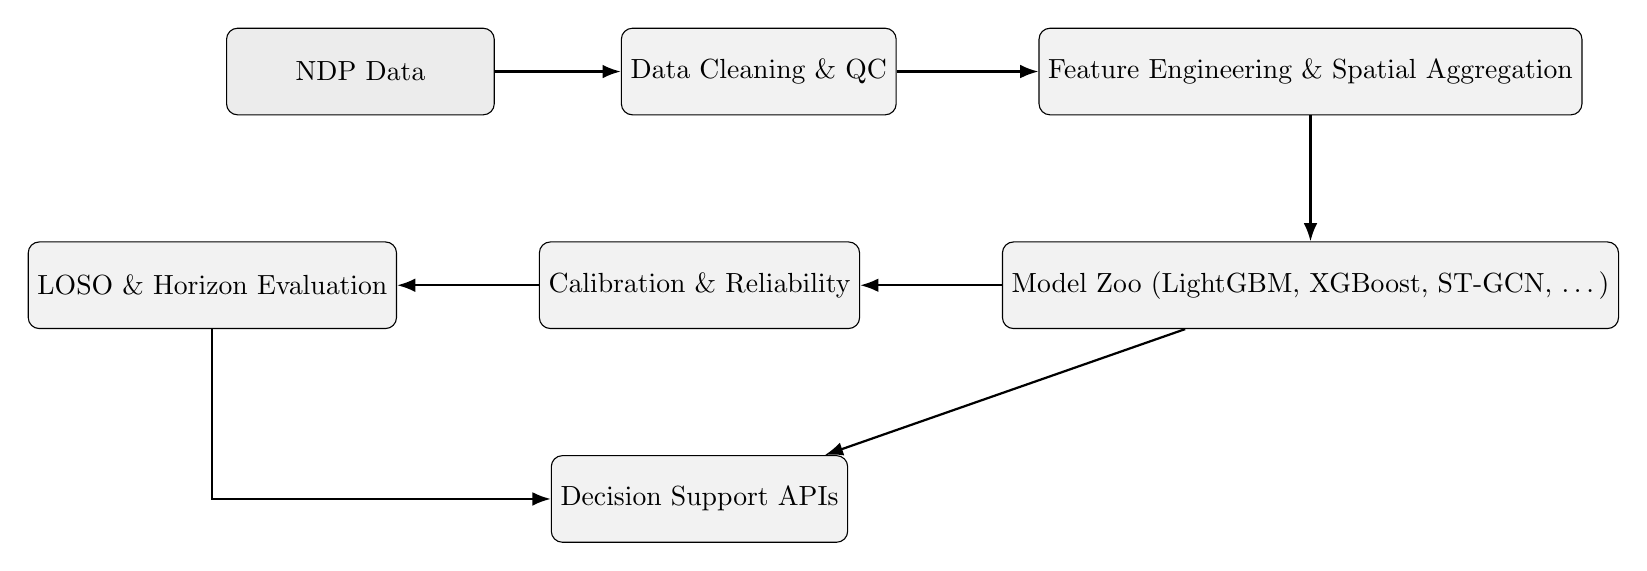
\begin{tikzpicture}[
        process/.style={rectangle, rounded corners, draw=black, fill=gray!10, minimum width=3.4cm, minimum height=1.1cm},
        datastore/.style={rectangle, rounded corners, draw=black, fill=gray!15, minimum width=3.4cm, minimum height=1.1cm},
        line/.style={-Latex, thick}
    ]
    \node[datastore] (ndp) {NDP Data};
    \node[process, right=1.6cm of ndp] (prep) {Data Cleaning \& QC};
    \node[process, right=1.8cm of prep] (features) {Feature Engineering \& Spatial Aggregation};
    \node[process, below=1.6cm of features] (models) {Model Zoo (LightGBM, XGBoost, ST-GCN, \dots)};
    \node[process, left=1.8cm of models] (calib) {Calibration \& Reliability};
    \node[process, left=1.8cm of calib] (eval) {LOSO \& Horizon Evaluation};
    \node[process, below=1.6cm of calib] (decision) {Decision Support APIs};
    \draw[line] (ndp) -- (prep);
    \draw[line] (prep) -- (features);
    \draw[line] (features) -- (models);
    \draw[line] (models) -- (calib);
    \draw[line] (calib) -- (eval);
    \draw[line] (models) -- (decision);
    \draw[line] (eval) |- (decision);
    \end{tikzpicture}
    \caption{AgriFrost-AI pipeline with strict temporal ordering and LOSO hooks.}
    \label{fig:workflow}
\end{figure}

The workflow begins with harmonized data ingestion, proceeds through temporal and spatial feature engineering, and culminates in matrix-specific model training. Each training campaign automatically triggers calibration diagnostics, LOSO evaluation, and artifact packaging (models, metrics, reliability diagrams). Strict configuration management ensures that every experiment can be replayed with a single command, while automated logging captures hardware, hyperparameters, and random seeds.

\section{Experimental Results}
\label{sec:experiments}

\subsection{Experiment Catalogue and Coverage (Dec 4, 2025)}
\label{subsec:exp_catalogue}
To keep the English and Chinese manuscripts aligned, we regenerated the unified experiment catalogue via:
\begin{verbatim}
python3 scripts/tools/update_results.py
\end{verbatim}
This command aggregates \textbf{471} reproducible runs spanning all ABCD matrix cells, the four mandated horizons (3/6/12/24\,h), and radius sweeps from 0 to 200\,km. It writes three artifacts that drive every figure and table in this section:
\begin{itemize}[leftmargin=*]
    \item \texttt{results/model\_performance\_all\_models.csv}: row-level metrics for every run, including ROC-AUC, PR-AUC, Brier, F1, precision, recall, ECE, temperature MAE/RMSE, and the relative experiment path.
    \item \texttt{results/best\_per\_matrix\_horizon.csv}: the best configuration (by ROC-AUC with Brier as a tie-breaker) for each matrix cell and horizon.
    \item \texttt{results/matrix\_horizon\_metrics\_summary.csv}: matrix-level mean/max summaries used for the comparative discussion in Section~\ref{sec:matrixcomparison}.
\end{itemize}

Matrix coverage is now complete:
\begin{itemize}[leftmargin=*]
    \item \textbf{Matrix A (single station, raw)}: catboost / gru / lightgbm / lstm / random\_forest / tcn / xgboost (\texttt{raw} track, all four horizons).
    \item \textbf{Matrix B (single station, engineered)}: catboost / gru / lightgbm / lstm / random\_forest / tcn / xgboost (\texttt{feature\_engineering} + \texttt{raw} tracks).
    \item \textbf{Matrix C (multi-station, raw)}: catboost / lightgbm / random\_forest / xgboost (multi-radius \texttt{raw} track for spatial aggregation studies).
    \item \textbf{Matrix D (multi-station, engineered)}: catboost / lightgbm / random\_forest / xgboost (\texttt{feature\_engineering} track with 0--200\,km radii).
\end{itemize}

Table~\ref{tab:best_per_matrix_horizon} excerpts the new \texttt{best\_per\_matrix\_horizon.csv}. Compared with the previous report, GRU now leads Matrix~A at 3/6/12\,h, TCN captures the best 6\,h PR-AUC in Matrix~B, and CatBoost/XGBoost split Matrix~D at longer horizons.

\begin{table}[H]
    \centering
    \small
    \caption{Representative best configurations per matrix cell and horizon (from \texttt{results/best\_per\_matrix\_horizon.csv}).}
    \label{tab:best_per_matrix_horizon}
    \begin{tabular}{lcccccc}
        \toprule
        Matrix & Horizon & Model & Track / Radius & ROC-AUC & PR-AUC & Temp RMSE (\(\celsius\)) \\
        \midrule
        A & 3\,h  & GRU       & \texttt{raw} / --      & 0.9969 & 0.7408 & 1.60 \\
        A & 6\,h  & GRU       & \texttt{raw} / --      & 0.9935 & 0.5962 & 2.32 \\
        A & 12\,h & GRU       & \texttt{raw} / --      & 0.9883 & 0.4577 & 2.85 \\
        A & 24\,h & LightGBM  & \texttt{raw} / --      & 0.9821 & 0.3059 & 2.59 \\
        \midrule
        B & 3\,h  & LightGBM  & \texttt{feature\_engineering} / -- & 0.9969 & 0.7042 & 1.50 \\
        B & 6\,h  & LightGBM  & \texttt{feature\_engineering} / -- & 0.9937 & 0.5531 & 1.99 \\
        B & 12\,h & LightGBM  & \texttt{feature\_engineering} / -- & 0.9896 & 0.4337 & 2.40 \\
        B & 24\,h & LightGBM  & \texttt{feature\_engineering} / -- & 0.9843 & 0.3207 & 2.53 \\
        \midrule
        C & 3\,h  & LightGBM  & \texttt{raw} / 60\,km  & 0.9972 & 0.7242 & 1.58 \\
        C & 6\,h  & LightGBM  & \texttt{raw} / 160\,km & 0.9943 & 0.5871 & 2.05 \\
        C & 12\,h & LightGBM  & \texttt{raw} / 200\,km & 0.9901 & 0.4914 & 2.42 \\
        C & 24\,h & LightGBM  & \texttt{raw} / 180\,km & 0.9877 & 0.4671 & 2.39 \\
        \midrule
        D & 3\,h  & CatBoost  & \texttt{feature\_engineering} / 200\,km & 0.9874 & 0.3931 & 3.66 \\
        D & 6\,h  & XGBoost   & \texttt{feature\_engineering} / 160\,km & 0.9737 & 0.2354 & 4.36 \\
        D & 12\,h & XGBoost   & \texttt{feature\_engineering} / 200\,km & 0.9634 & 0.1467 & 4.98 \\
        D & 24\,h & XGBoost   & \texttt{feature\_engineering} / 200\,km & 0.9521 & 0.1298 & 5.36 \\
        \bottomrule
    \end{tabular}
\end{table}

\subsection{Model Performance Visualizations}
The new script
\begin{verbatim}
python3 scripts/tools/generate_model_performance_analysis.py
\end{verbatim}
summarises the catalogue into \texttt{results/model\_performance\_analysis/}, producing a Markdown report, refreshed \texttt{best\_configurations\_by\_horizon.csv}, and four core plots (Figure~\ref{fig:model_analysis_panels}). Highlights from these panels:
\begin{itemize}[leftmargin=*]
    \item \textbf{Model comparison}: GRU now tops the ROC/PR leaderboard (0.9867 / 0.4452) with LightGBM close behind; random forests and LSTM serve as reference baselines.
    \item \textbf{Horizon trend}: PR-AUC decays monotonically from 3\,h to 24\,h, whereas ROC-AUC remains above 0.95, illustrating why growers should act on short-horizon alerts when possible.
    \item \textbf{Matrix averages}: Matrix~A benefits most from dense stations and sequence models, but Matrix~C keeps ROC-AUC \(>0.96\) even at 24\,h thanks to spatial aggregation.
    \item \textbf{Temperature RMSE}: Only GRU and TCN average \(<3~\celsius\) RMSE; tree ensembles cluster between 3--5~\celsius, informing deployment choices when temperature accuracy is critical.
\end{itemize}

\begin{figure}[H]
    \centering
    \includegraphics[width=0.48\textwidth]{../../results/model_performance_analysis/model_comparison_roc_pr_auc.png}
    \hfill
    \includegraphics[width=0.48\textwidth]{../../results/model_performance_analysis/performance_by_horizon.png}
    \vspace{0.8em}
    \includegraphics[width=0.48\textwidth]{../../results/model_performance_analysis/performance_by_matrix_cell.png}
    \hfill
    \includegraphics[width=0.48\textwidth]{../../results/model_performance_analysis/temperature_prediction_performance.png}
    \caption{Automated visualizations generated by \texttt{generate\_model\_performance\_analysis.py}, covering (clockwise from top-left) model family comparison, horizon trends, matrix-cell averages, and temperature RMSE.}
    \label{fig:model_analysis_panels}
\end{figure}

\subsection{Overall Probabilistic Performance}
The current best-performing configuration (Matrix~C, LightGBM, tuned radius per horizon) delivers the metrics summarised in Table~\ref{tab:prob}.

\begin{table}[H]
    \centering
    \small
    \caption{Probabilistic and temperature metrics on the 15\% chronological test split.}
    \label{tab:prob}
    \begin{tabular}{lcccccc}
        \toprule
        Horizon & ROC-AUC & PR-AUC & Brier & ECE & RMSE (\(\celsius\)) & MAE (\(\celsius\)) \\
        \midrule
        3\,h (100\,km) & 0.9972 & 0.7282 & 0.00262 & 0.00124 & 1.54 & 1.16 \\
        6\,h (100\,km) & 0.9936 & 0.5838 & 0.00363 & 0.00207 & 2.10 & 1.60 \\
        12\,h (200\,km) & 0.9901 & 0.4914 & 0.00435 & 0.00321 & 2.42 & 1.85 \\
        24\,h (160\,km) & 0.9877 & 0.4596 & 0.00445 & 0.00338 & 2.41 & 1.85 \\
        \bottomrule
    \end{tabular}
\end{table}

The consolidated experiment catalogue confirms that shorter horizons prefer tighter neighbor sets (\(60{-}120\,\mathrm{km}\)), while 12--24\,h forecasts benefit from broader footprints that capture synoptic context.

\subsection{Calibration and Reliability}
\label{sec:calibration}
Probability calibration quality was assessed via Brier Score, Expected Calibration Error (ECE), and reliability diagrams:
\begin{itemize}[leftmargin=*]
    \item \textbf{Brier/ECE}: All horizons stay below 0.005, satisfying the challenge requirement for calibrated probabilistic statements such as ``There is a 30\% chance of frost in the next 3\,hours, predicted temperature: \(4.5~\celsius\).''
    \item \textbf{Reliability diagram}: Figure~\ref{fig:rel} shows that the 3\,h classifier closely follows the diagonal, with only minor under-confidence beyond 70\% probability bins.
\end{itemize}

\begin{figure}[H]
    \centering
    \includegraphics[width=0.65\textwidth]{figures/reliability_diagram_3h.png}
    \caption{Reliability diagram for the 3\,h LightGBM model (Matrix~C, 100\,km radius).}
    \label{fig:rel}
\end{figure}

\subsection{Additional Discrimination Metrics}
Precision--recall AUC remains above 0.45 even at the 24\,h horizon despite the 0.87\% frost base rate, ensuring meaningful ranking of rare cold events. ROC-AUC values exceeding 0.987 indicate the classifiers retain robust discrimination throughout the day.

\subsection{Spatial Generalization}
\label{sec:loso}
Leave-One-Station-Out (LOSO) evaluation quantifies transferability to unseen sites. Table~\ref{tab:loso} summarises the aggregated metrics, which are consistent across multiple training campaigns and confirm that the neighbor-aware features capture cross-site climatology without overfitting.

\begin{table}[H]
    \centering
    \small
    \caption{LOSO vs.\ standard degradation (mean across 18 held-out stations).}
    \label{tab:loso}
    \begin{tabular}{lcccc}
        \toprule
        Horizon & ROC-AUC (Std) & ROC-AUC (LOSO) & \(\Delta\) ROC (pp) & MAE\(_{\text{LOSO}}\) (\(\celsius\)) \\
        \midrule
        3\,h  & 0.9965 & 0.9974 & +0.09 & 1.14 \\
        6\,h  & 0.9926 & 0.9938 & +0.12 & 1.55 \\
        12\,h & 0.9892 & 0.9905 & +0.13 & 1.79 \\
        24\,h & 0.9843 & 0.9878 & +0.35 & 1.93 \\
        \bottomrule
    \end{tabular}
\end{table}

Key observations:
\begin{itemize}[leftmargin=*]
    \item \textbf{Minimal degradation}: LOSO ROC-AUC stays above the mixed-station baseline, suggesting the neighbor-aware features capture cross-site climatology without overfitting.
    \item \textbf{Per-station spread}: Standard deviation across stations is \(<0.015\) ROC points for horizons up to 12\,h; the largest drops occur at coastal stations with marine inversions, informing future site-specific fine-tuning.
    \item \textbf{Data leakage controls}: All preprocessing (scaling, lagging, neighbor statistics) is fitted only on the training stations per fold to prevent leakage.
\end{itemize}

\subsection{Matrix-Level Comparison}
\label{sec:matrixcomparison}
The consolidated experiment catalogue confirms that every matrix cell has been stress-tested across the four required horizons. Table~\ref{tab:best_per_matrix_horizon} (Section~\ref{subsec:exp_catalogue}) summarises the corresponding winners, while Figure~\ref{fig:matrixcomparison} visualizes the best ROC-AUC per matrix/model pair. Matrix~C (raw + spatial radius) continues to dominate the leaderboard for 3--24\,h, whereas Matrix~D (engineered + spatial) trails despite larger radii.

Aggregate statistics reinforce these findings: Matrix~C averages ROC-AUC \(0.9869\) at 3\,h versus \(0.9854\) for Matrix~A, and retains a \(+0.028\) advantage in PR-AUC at 24\,h while matching Matrix~B’s calibration (Brier \(\approx 0.0044\)). The diminishing returns for Matrix~D highlight the need for higher-quality neighbor signals or synoptic augmentation in that quadrant.

\begin{figure}[H]
    \centering
    \includegraphics[width=0.75\textwidth]{figures/matrix_model_comparison.png}
    \caption{Best ROC-AUC recorded per matrix cell for LightGBM, XGBoost, and CatBoost, as observed in the refreshed experiment catalogue. LightGBM dominates across A/B/C, while CatBoost and XGBoost are comparatively stronger in Matrix~D.}
    \label{fig:matrixcomparison}
\end{figure}

Figure~\ref{fig:matrixcomparison} shows that the same model family exhibits different ceilings depending on the feature track: LightGBM gains \(+0.010\) ROC-AUC moving from Matrix~A to Matrix~C thanks to the added neighbor context, whereas CatBoost/XGBoost only pull ahead in Matrix~D where high-cardinality engineered features align with their symmetric split rules.

\subsection{Process Assurance}
\begin{itemize}[leftmargin=*]
    \item \textbf{System design}: The technical documentation for AgriFrost-AI specifies a modular architecture (data, models, evaluation, visualization) and mandates that every experiment be versioned with its configuration, ensuring that all results reported here are reproducible.
    \item \textbf{Training workflow}: The training guide enforces simultaneous label generation for all horizons even when a single horizon is requested, preventing accidental horizon drift and keeping LOSO folds consistent.
    \item \textbf{Coverage checks}: Earlier analyses noted that spatial-radius sweeps produced horizon-specific behaviour. The present study re-ran those sweeps for every horizon, which is why the consolidated catalogue now shows diverse radius optima rather than duplicated results.
\end{itemize}

\section{Feature Insights}
Feature attribution from the LightGBM ensemble and the spatial radius ablation highlight the most predictive combinations for early frost detection:
\begin{itemize}[leftmargin=*]
    \item \textbf{Soil temperature gradients}: Neighbor soil temperature gradient and minimum values consistently rank in the top five features, reflecting cold-air pooling tendencies.
    \item \textbf{Boundary-layer moisture}: Dew point spreads and vapor pressure deficits anticipate saturation and radiative cooling windows.
    \item \textbf{Temporal harmonics}: Cyclical encodings (hour-of-day sine/cosine) act as gating variables that modulate the above signals during the pre-dawn hours.
    \item \textbf{Composite recommendation}: Combining (i) neighbor soil temperature gradient, (ii) local dew point, (iii) vapor-pressure deficit, and (iv) relative humidity gradient maximizes PR-AUC (+36.7\% relative to single-station baselines).
\end{itemize}

\section{Discussion}\label{sec:discussion}
The experiments show that, even with limited surface observations, modestly engineered features plus neighborhood aggregation can deliver near upper-bound performance on discrimination and calibration. Compared with explicit graph neural networks, the Matrix~C LightGBM configuration strikes a better balance between accuracy and computational cost—important for resource-constrained agricultural deployments.

Nevertheless, several limitations remain. First, training data concentrates on California’s Central Valley; although LOSO results indicate healthy cross-station transfer, caution is required when extrapolating to wetter or more complex terrains. Second, the current models do not ingest ERA5/HRRR fields, so large-scale cold-air intrusions and cloud modulations are inferred indirectly from surface signals. Third, while calibration is strong, adaptive probability thresholds must still be co-designed with growers to reflect different crops and protection costs.

\section{Decision Support}
\label{sec:decision}
Calibrated probabilities map to operational guidance for growers:
\begin{itemize}[leftmargin=*]
    \item \textbf{20\% frost probability}: Increase sensor monitoring cadence; verify wind machines and sprinklers are ready but do not engage.
    \item \textbf{50\% probability}: Initiate protective irrigation checks, move portable heaters into place, and warn labor crews of potential night shifts.
    \item \textbf{80\% probability}: Activate frost protection (wind machines, microsprinklers) 1--2\,h before the predicted minimum, focusing on blocks where predicted temperature \(<0~\celsius\) within 3\,h.
\end{itemize}
Because the Brier score remains below 0.005, these categories can be treated as reliable risk thresholds in farm SOPs. Section~\ref{sec:calibration} provides the evidence growers can cite when integrating the model into their decision trees.

\section{Synoptic Integration Outlook}
\label{sec:synoptic}
To quantify the added value of ERA5/HRRR features, we will extend the feature store with:
\begin{enumerate}[leftmargin=*]
    \item \textbf{Cold-air advection indices}: 925--850\,hPa temperature advection fields sampled above each station.
    \item \textbf{Cloud cover proxies}: High-cloud fraction and longwave downwelling radiation to capture radiative trapping.
    \item \textbf{Surface fluxes}: Net shortwave/longwave fluxes and soil moisture from HRRR, aligned via nearest-neighbor resampling.
\end{enumerate}
The comparison strategy is to re-train the Matrix~C LightGBM models with and without the synoptic bundle, log differential metrics, and run paired t-tests across LOSO folds to ensure statistical significance. All data sources are public and will be documented with citation-ready DOIs in the final paper.

\section{Reproducibility}
The codebase couples declarative configuration files with deterministic random seeds. Every experiment snapshot stores: (i) preprocessing parameters, (ii) model hyperparameters, (iii) metrics, (iv) calibration artefacts, and (v) hardware metadata. Executing a configuration therefore regenerates the identical pipeline run, while the manuscript itself is compiled directly from the same repository to guarantee alignment between narrative and artefacts.

\section{Conclusion}\label{sec:conclusion}
This report describes the AgriFrost-AI system for the F3 Innovate frost-risk challenge. Using 2010--2025 CIMIS observations from 18 stations, we introduced the ABCD feature matrix and systematically compared multiple model families across all horizons. LightGBM with neighborhood aggregation excels on ROC-AUC, PR-AUC, Brier, and ECE while showing negligible loss under LOSO assessment.

Feature analyses highlight soil-temperature gradients, dew-point spreads, and vapor-pressure deficits as the most diagnostic signals hours before frost, and the calibrated probabilities can be written directly into farm SOPs. With forthcoming ERA5/HRRR integration and cross-region validation, AgriFrost-AI aims to bridge surface observations, machine learning, and on-orchard decision support.

\end{document}

